\chapter{Исходная программа и методика измерений}

\section{Архиватор MZ77}

MZ77 "--- программа для операционных систем семейства GNU/Linux. Пользователь
выбирает в окне программы (рисунок~\ref{fig:window}) исходные файлы, режим
работы (сжатие или распаковка) и каталог для результатов. Файлы
обрабатываются рабочими потоками POSIX; каждый файл сжимается функцией
\texttt{lz77\_compress} и распаковывается функцией
\texttt{lz77\_decompress} из файла \texttt{src/lz77.c}. Побитовая запись и
чтение архива выполняются функциями из \texttt{src/bitio.c}. Графический
интерфейс в работе не оптимизируется: всё время работы программы приходится
на эти две функции.

\begin{figure}[H]
  \centering
  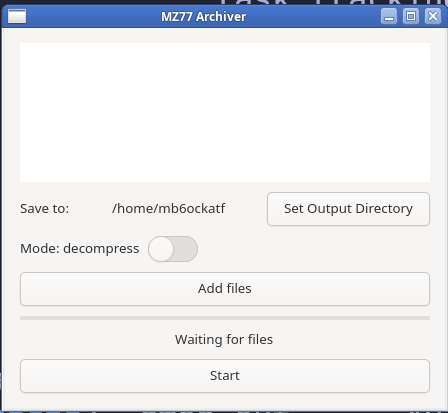
\includegraphics[width=0.7\textwidth]{pic/window.png}
  \caption{Окно архиватора MZ77}
  \label{fig:window}
\end{figure}

Алгоритм LZ77~\cite{ziv-lempel} заменяет повторяющиеся фрагменты входных
данных ссылками на их предыдущие вхождения. Сжатие идёт по входному файлу
слева направо. В~каждой позиции программа ищет в~\emph{окне} "--- последних
4096 обработанных байтах "--- самую длинную строку, совпадающую с началом
\emph{упреждающего буфера} (ещё не сжатых данных). Если найдено совпадение
длиной не менее 3~байт, в архив записывается ссылка (смещение, длина),
иначе "--- один байт как литерал. Ссылка или литерал называется
\emph{токеном}. Формат токенов архива MZ77 приведён в
таблице~\ref{tab:format}.

\begin{table}[H]
\caption{Формат токенов архива MZ77}
\label{tab:format}
\begin{tabletext}
\centering
\begin{tabular}{|l|l|l|l|}
\hline
\textbf{Токен} & \textbf{Флаг} & \textbf{Поля} & \textbf{Всего бит} \\
\hline
Литерал & 1 бит, 0 & байт данных, 8 бит & 9 \\
\hline
Ссылка & 1 бит, 1 & смещение $-1$, 12 бит; длина $-3$, 8 бит & 21 \\
\hline
\end{tabular}
\end{tabletext}
\end{table}

Для быстрого поиска совпадений используется хеш-таблица с цепочками.
Хеш трёх первых байт позиции выбирает голову цепочки
(\texttt{ht\_heads}, 65\,536 голов); массив \texttt{ht\_next} размером с
окно связывает каждую позицию с предыдущей позицией с тем же хешем.
Поиск проходит не более 256 позиций цепочки и прекращается при совпадении
максимальной длины "--- 258 байт (те же пределы длины совпадения, что и в
формате DEFLATE~\cite{deflate}). Параметры алгоритма приведены в
таблице~\ref{tab:params}; они не менялись ни на одном шаге оптимизации,
поэтому коэффициент сжатия на всех шагах одинаков.

\begin{table}[H]
\caption{Параметры алгоритма сжатия}
\label{tab:params}
\begin{tabletext}
\centering
\begin{tabular}{|l|c|l|}
\hline
\textbf{Параметр} & \textbf{Обозначение} & \textbf{Значение} \\
\hline
Размер окна & $W$ & 4096 байт \\
Размер упреждающего буфера & $L$ & 4096 байт \\
Минимальная длина совпадения & $M_{\min}$ & 3 байта \\
Максимальная длина совпадения & $M$ & 258 байт \\
Число голов хеш-таблицы & $H$ & 65\,536 \\
Максимальная длина просматриваемой цепочки & $C$ & 256 позиций \\
\hline
\end{tabular}
\end{tabletext}
\end{table}

\section{Тестовые компьютеры}

Измерения проводились на двух компьютерах (таблица~\ref{tab:machines}).
Процессор AMD поддерживает векторные команды AVX2, процессор Intel "---
также AVX-512. Это позволило проверить каждую машинно-зависимую
оптимизацию на процессоре, для которого она предназначена, и убедиться, что
на другом процессоре она ничего не ухудшает. Результаты двух компьютеров
между собой не сравниваются: сравниваются только шаги оптимизации на одном
компьютере.

\begin{table}[H]
\caption{Тестовые компьютеры}
\label{tab:machines}
\begin{tabletext}
\centering
\begin{tabular}{|l|l|l|}
\hline
 & \textbf{debian} & \textbf{hppavillion} \\
\hline
Процессор & AMD Ryzen 7 5700U & Intel Core i3-1115G4 \\
Микроархитектура & Zen 2 & Tiger Lake \\
Ядра / потоки & 8 / 16 & 2 / 4 \\
Векторные расширения & AVX2 & AVX2, AVX-512BW \\
Оперативная память & 30 ГБ & 7,4 ГБ \\
Операционная система & Debian 13 & Devuan 6 (на базе Debian 13) \\
Ядро Linux & 6.12 & 6.12 \\
Компилятор & GCC 14.2 & GCC 16.2 \\
\hline
\end{tabular}
\end{tabletext}
\end{table}

\screenshot{machines}{Характеристики процессоров тестовых компьютеров}{fig:machines}{%
Два окна терминала рядом: на каждом компьютере выполнить
\texttt{lscpu | head -20} и \texttt{gcc --version | head -1}.}

\section{Набор тестовых данных}

Для измерений использован корпус Silesia~\cite{silesia} "--- 12 файлов
реальных данных общим объёмом 211~МБ, стандартный набор для оценки
архиваторов общего назначения, "--- и четыре синтетических файла по 20~МБ,
которые программа тестирования генерирует с фиксированным начальным
значением генератора случайных чисел (таблица~\ref{tab:corpus}). Всего
корпус содержит 16 файлов и 291~МБ.

\begin{table}[H]
\caption{Набор тестовых данных}
\label{tab:corpus}
\begin{tabletext}
\centering
\begin{tabular}{|l|r|l|}
\hline
\textbf{Файл} & \textbf{Размер, МБ} & \textbf{Содержимое} \\
\hline
text.dat & 20,0 & синтетический английский текст \\
random.dat & 20,0 & случайные байты: несжимаемые данные \\
zeros.dat & 20,0 & нулевые байты: самые длинные совпадения \\
mixed.dat & 20,0 & короткая фраза, каждый восьмой байт случаен \\
\hline
dickens & 10,2 & произведения Ч.~Диккенса, английский текст \\
mozilla & 51,2 & исполняемые файлы Mozilla 1.0 \\
mr & 10,0 & медицинское изображение МРТ \\
nci & 33,6 & база данных химических структур \\
ooffice & 6,2 & динамическая библиотека OpenOffice.org \\
osdb & 10,1 & тестовая база данных MySQL \\
reymont & 6,6 & текст на польском языке \\
samba & 21,6 & исходные тексты Samba \\
sao & 7,3 & каталог звёзд SAO, двоичный \\
webster & 41,5 & словарь Уэбстера, HTML \\
x-ray & 8,5 & рентгеновский снимок \\
xml & 5,3 & набор XML-файлов \\
\hline
\end{tabular}
\end{tabletext}
\end{table}

\section{Методика измерений}

Графический интерфейс в измерениях не участвует. Программа тестирования
\texttt{bench/mz77-bench} вызывает функции \texttt{lz77\_compress} и
\texttt{lz77\_decompress} напрямую, запускает каждый файл несколько раз и
сообщает медиану времени по часам \texttt{CLOCK\_MONOTONIC}, скорость в
МБ/с и коэффициент сжатия. Временные архивы пишутся в \texttt{/dev/shm},
чтобы диск не вносил шума. При первом запуске каждого файла программа
распаковывает архив и сравнивает результат с исходным файлом.

Для каждого шага оптимизации выполнялись:
\begin{itemize}
\item сборка в конфигурации выпуска (\texttt{./configure --enable-release}:
\texttt{-O3 -DNDEBUG -fhardened}) и набор тестов \texttt{make check};
\item измерение времени сжатия и распаковки всего корпуса, медиана из
9~запусков (\texttt{bench/campaign.sh});
\item профилирование одного файла (dickens) инструментами gprof~\cite{gprof},
perf~\cite{perf} и Valgrind (Cachegrind, Callgrind)~\cite{valgrind};
программа для профилирования собирается с одними и теми же флагами
\texttt{-O2 -g} на всех шагах;
\item проверка того, что архивы всех файлов корпуса совпадают байт в байт с
архивами исходной программы (контрольные суммы SHA-256).
\end{itemize}

Время работы на ноутбуке оказалось ненадёжной мерой: его процессор менял
тактовую частоту между запусками до 40~\%. Поэтому основной мерой
производительности в отчёте служит число тактов процессора в
пользовательском режиме (событие \texttt{cycles:u} счётчика
\texttt{perf~stat}), которое от частоты не зависит. В~конце работы
сценарий \texttt{bench/steps.sh} заново собрал программу каждого шага из
её коммита и измерил все шаги подряд, чередуя их, на одном закреплённом
ядре процессора (\texttt{taskset}), по пять раундов; в отчёте приводится
медиана. Число выполненных команд (\texttt{instructions:u}) не зависит ни
от частоты, ни от фоновой нагрузки и используется для оценки сложности.
Время в секундах приводится для компьютера debian, частота которого во
время измерений была стабильной.

Ускорение шага записывается как отношение $k = T_{\text{до}} /
T_{\text{после}}$: значение $1{,}52\times$ означает, что программа работает
в~1,52~раза быстрее, то есть затрачивает на $1 - 1/1{,}52 = 34~\%$ меньше
тактов.

\section{Последовательность оптимизаций}

Оптимизации выполнялись по одной; после каждой программа проверялась,
измерялась и профилировалась, а изменения фиксировались отдельным коммитом
в ветке \texttt{dev} репозитория~\cite{mz77-repo}. Шаги перечислены в
таблице~\ref{tab:steps} в порядке выполнения. В~главах~3--5 они
сгруппированы по виду оптимизации, как того требует задание; сравнение
<<до>> и <<после>> в каждом разделе ведётся с предыдущим по времени шагом.

\begin{table}[H]
\caption{Шаги оптимизации в порядке выполнения}
\label{tab:steps}
\begin{tabletext}
\centering
\begin{tabular}{|c|l|l|l|c|}
\hline
\textbf{Шаг} & \textbf{Изменение} & \textbf{Вид} & \textbf{Коммит} & \textbf{Раздел} \\
\hline
00 & исходная программа & "--- & 1f70c33 & 2 \\
01 & блочный ввод-вывод & машинно-независимая & cc7a482 & 4.1 \\
02 & встраивание побитового ввода-вывода & машинно-независимая & 08b2ec5 & 4.2 \\
03 & общий буфер окна, без сдвига & алгоритмическая & c1c1f4a & 3 \\
04 & сравнение по 8 байт & машинно-независимая & c1c1f4a & 4.3 \\
05 & сравнение командами AVX-512BW & машинно-зависимая & 02312cd & 5.1 \\
06 & сравнение командами AVX2 & машинно-зависимая & 55149a1 & 5.2 \\
07 & LTO и PGO & машинно-независимая & 5d53dc4 & 4.4 \\
\hline
\end{tabular}
\end{tabletext}
\end{table}
